\section{Design}

The PCAL geometry~\cite{2015002} is similar to the CLAS EC~\cite{clas6nim} and shown schematically in Figs. \ref{fig:S3_1} and \ref{fig:S3_2}.   The active area of PCAL is an isosceles triangle with a base length of $394$ cm and a base angle $\alpha=62.9^o$. The apex of the triangle is nearest the beamline. Each PCAL module is composed of 15 scintillator layers sandwiched with 14 layers of lead, similar to the inner calorimeter of the CLAS EC.  Each scintillator and lead layer is separated by a $50~\mu$m Teflon sheet and the entire scintillator/lead volume is confined within a triangular shaped box that has composite front and rear windows and aluminum side plates. Each window consists of $25.4$ mm thick foam (FR-3715 Last-A-Foam, density 0.24~g~cm$^{-3}$) sandwiched between $2$ mm thick stainless steel sheets and supported by a stainless steel frame on the perimeter.  Particles entering PCAL from the target will pass through the forward entrance window, layers of lead and scintillator, the rear exit window and the front entrance window of the EC.  The PCAL active area is slightly larger than the acceptance of the EC projected towards the CLAS target to the location of the last layer of the PCAL. 

\begin{figure}[hbt]
\centering
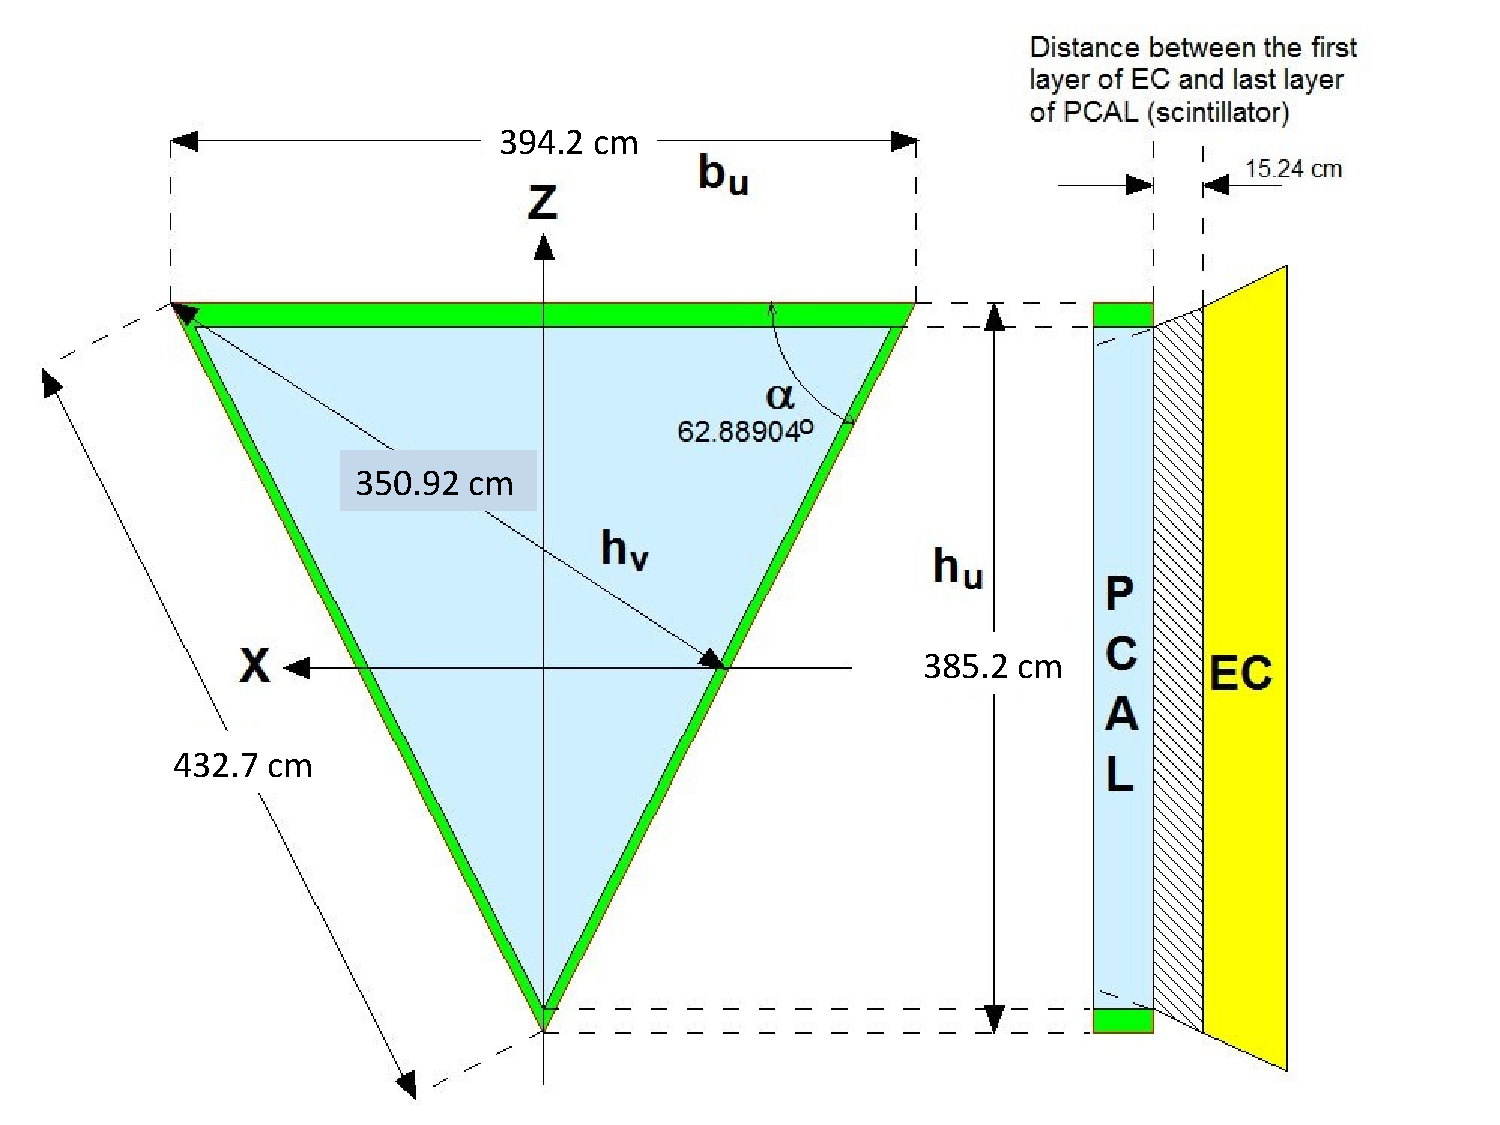
\includegraphics[width=1.0\columnwidth,keepaspectratio]{img/S3_1.pdf}
\caption[A schematic plot of PCAL]{A schematic plot showing the dimensions of a PCAL module. The design length $L_1$ of the longest scintillator strips are $L_1=394.2$~cm for the U strips and $L_1=432.7$~cm for the V and W strips. }
\label{fig:S3_1}
\end{figure}

The scintillator layers have three alternating stereo readout planes named U, V and W which are interleaved with layers of lead as illustrated in Fig. \ref{fig:S3_2}. The readout planes are divided into scintillator strips of varying lengths but with a fixed cross-sectional area of $4.5 \times 1$ cm$^2$. In each stereo readout layer the strips are oriented parallel to one of the sides of the triangle (Fig. \ref{fig:S2_2}). For the U-view, the strips are parallel to the base of the triangle, farthest from the beamline. For the W-view, the strips are parallel to the U PMT readout side.  For the V view, the strips are parallel to the last remaining side.  

\begin{figure}[hbt]
\centering
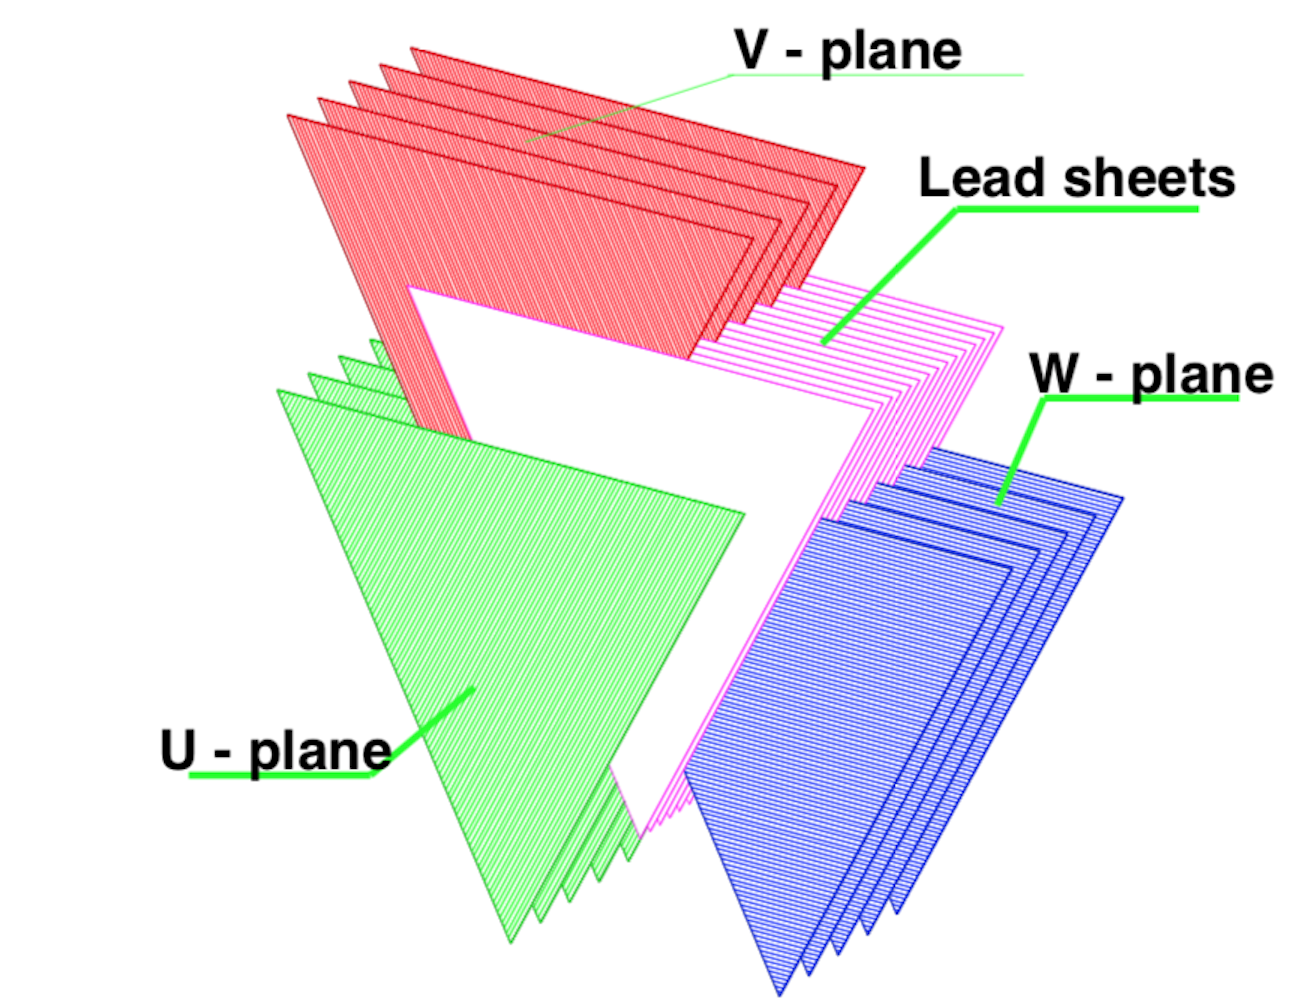
\includegraphics[width=0.95\columnwidth,keepaspectratio]{img/S3_2.png}
\caption[PCAL UVW Layers]{Schematic showing interleaving of U,V,W scintillator layers with lead. }
\label{fig:S3_2}
\end{figure}

Light generated in the scintillator strips by ionizing radiation is wavelength shifted using Kururay Y-11 $1$ mm diameter multi-clad fibers inserted inside holes along the strips (Fig. \ref{fig:S3_4}). The fibers also transport the light to the PMT housings located along the base and U readout side of the triangle. At the readout end, the fiber ends are milled, polished and coupled to the PMTs with optical grease (Fig. \ref{fig:S3_5}). The opposite ends of the fibers stick out from the far end of the strips by $\sim 1$ mm and are spot glued to the scintillator.

\begin{figure}[hbt]
\centering
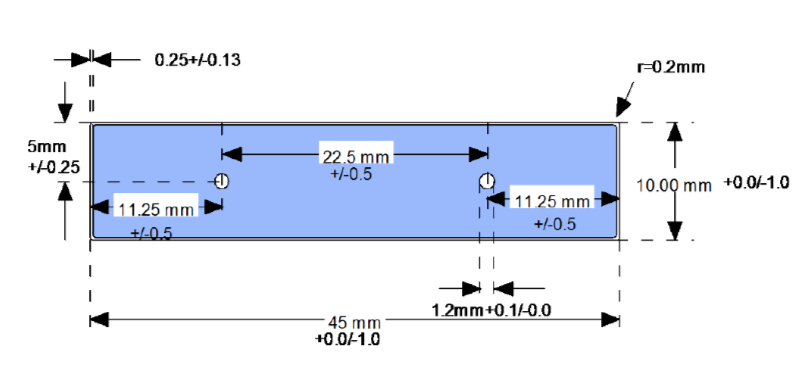
\includegraphics[width=1.05\columnwidth,keepaspectratio]{img/S3_4a.png}
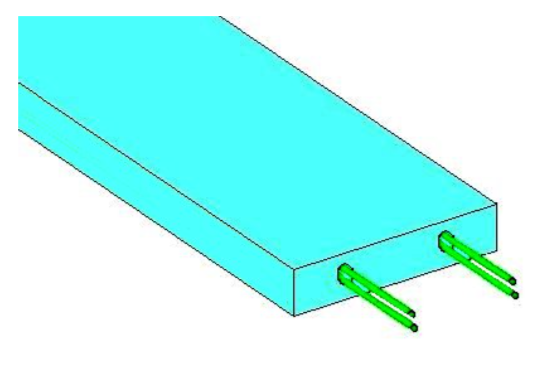
\includegraphics[width=0.75\columnwidth,keepaspectratio]{img/S3_4b.png}
\caption[PCAL UVW Layers]{Top: Designed dimensions of scintillator cross section Bottom: Rendering of the strip with two fibers in each hole}
\label{fig:S3_4}
\end{figure}

There are $84$ strips in the U-view, and $77$ strips in the V- and W-views. In order to optimize the number of readout channels, pair of strips at large scattering angles were combined into a single readout channel (fibers from two adjacent strips were routed to a single PMT).  For the first 52 shortest strips in U and for the last 46 longest strips in the V and W stereo readout planes the 45 mm (single strip) segmentation is used. For the
remaining strips, 90-mm wide (double strip) segmentation is used.  Thus there are a total of 68 PMT readout channels for U, and 62 for V and W.
\begin{figure}[hbt]
\centering
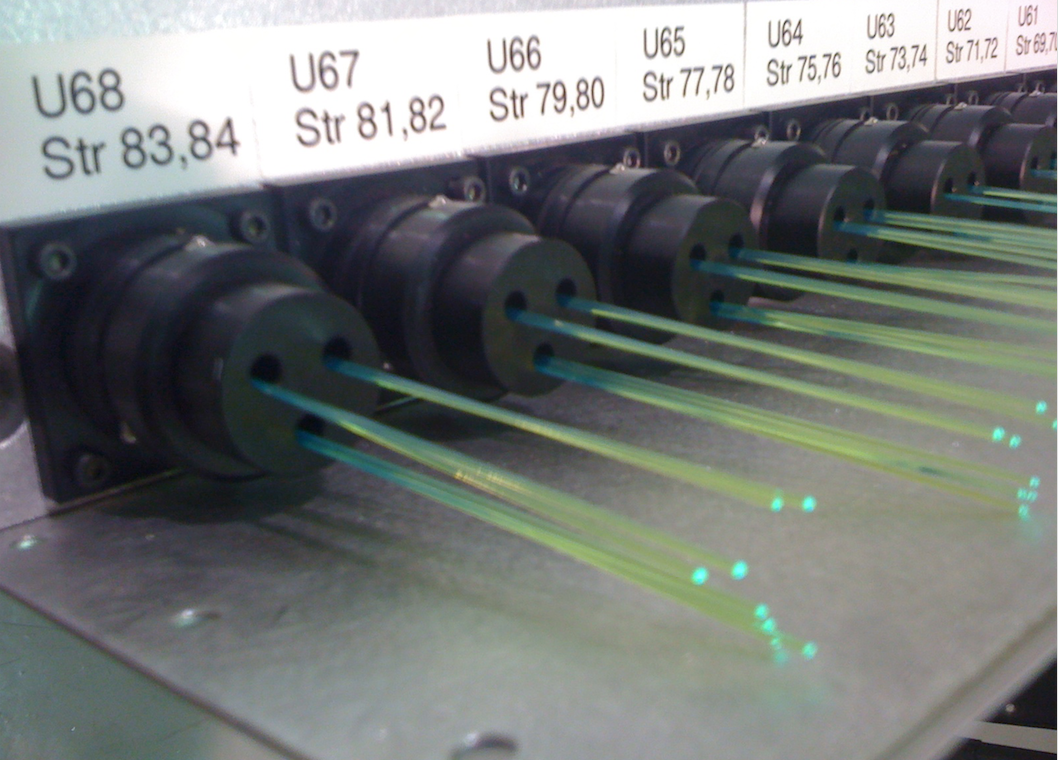
\includegraphics[width=0.9\columnwidth,keepaspectratio]{img/S3_5a.png}
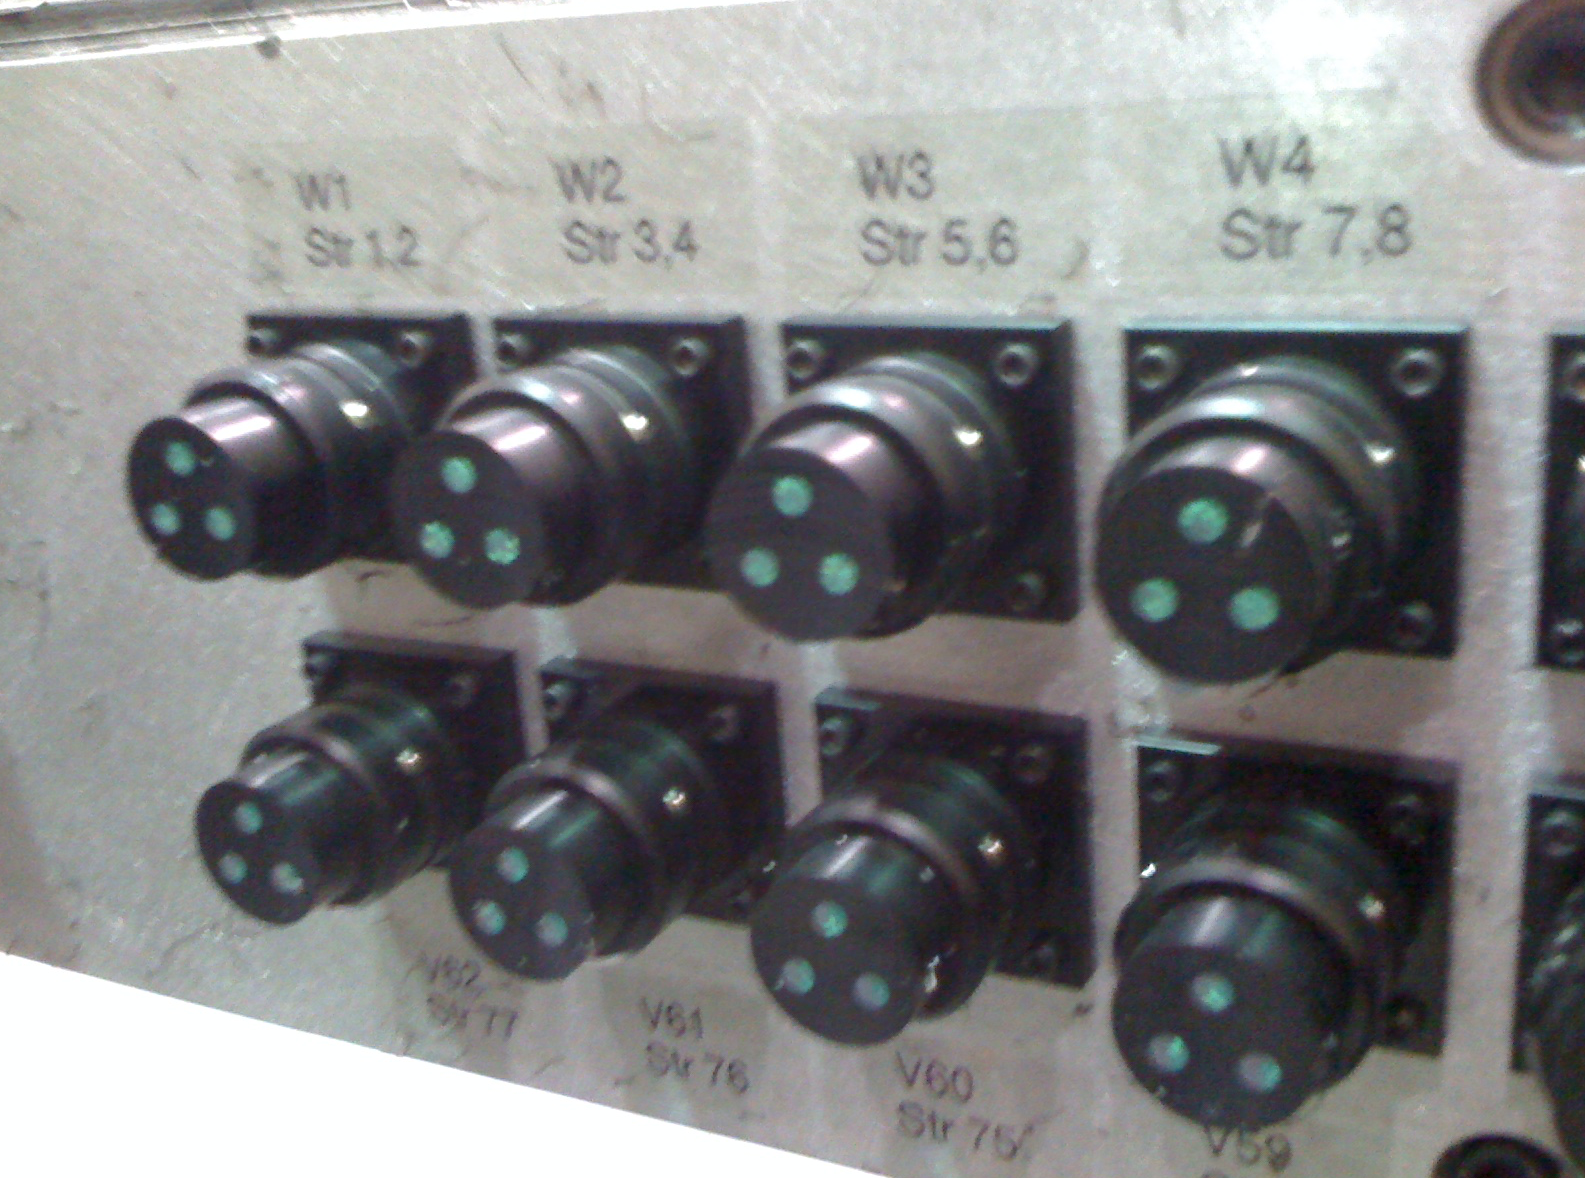
\includegraphics[width=0.9\columnwidth,keepaspectratio]{img/S3_5b.png}
\caption[PCAL UVW Layers]{Top: WLS fibers from scintillators extending from PMT housings. Bottom: WLS fibers after milling and polishing prior to PMT installation.}
\label{fig:S3_5}
\end{figure}

All lead and scintillator layers inside the box are held in position by a retaining assembly attached to two of the sidewalls.  These retainers also create a space between the sidewall and the end of the scintillator strips in order to route the light readout fibers out of the box to the PMT housings (Fig. \ref{fig:S3_3}). 

\begin{figure}[hbt]
\centering
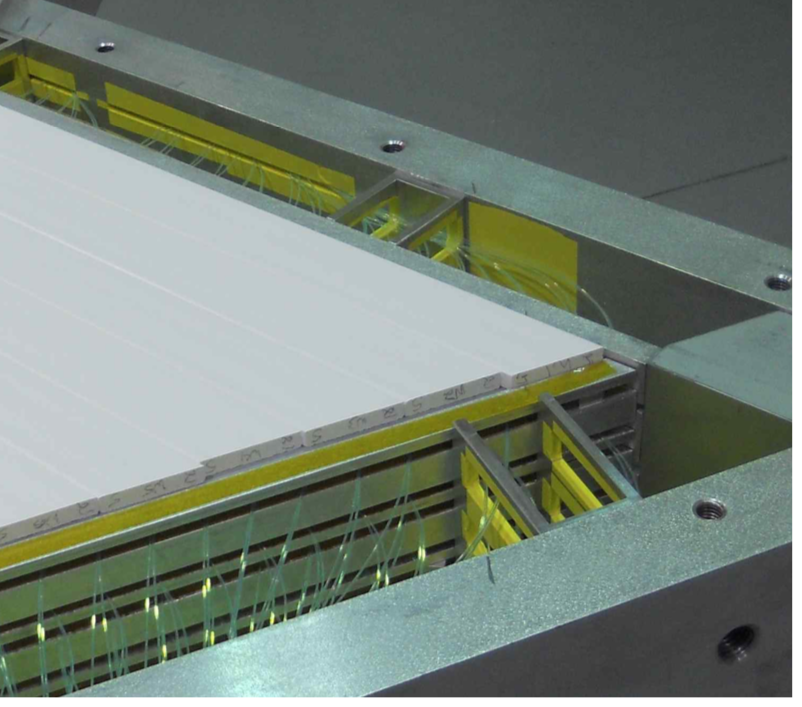
\includegraphics[width=0.95\columnwidth,keepaspectratio]{img/S3_6.png}
\caption[PCAL UVW Layers]{Retainer assembly at the corner of the back-side and U-PMT readout side.}
\label{fig:S3_3}
\end{figure}


